\documentclass[conference]{IEEEtran}
\usepackage{cite}
\usepackage{graphicx}
\usepackage{amsmath}
\usepackage{amssymb}
\usepackage{tikz}
\usetikzlibrary{shapes.geometric, arrows}
\begin{document}

\title{File System Management using Voice Assistant in Linux}

\author{
\IEEEauthorblockN{Jeyadev Needhidevan}
\IEEEauthorblockA{2021503020}
\and 
\IEEEauthorblockN{Ram Prasath G}
\IEEEauthorblockA{2021503544}
\and 
\IEEEauthorblockN{Deepesh Vikram K}
\IEEEauthorblockA{2021503014}
\and 
\IEEEauthorblockN{Vishnu G}
\IEEEauthorblockA{2021503570}
}

\maketitle

\begin{abstract}
In this paper, we present a novel approach for managing the file system in Linux using a voice assistant. Our proposed system allows users to perform file system operations such as creating directories, renaming files, and deleting files by issuing voice commands. We develop a voice assistant using Python libraries and integrate it with the file system in Linux. The voice assistant is capable of understanding natural language and executing commands based on the user's voice inputs. We conduct experiments to evaluate the performance of the system and demonstrate that our approach is effective and efficient in managing the file system using voice commands. Our proposed system can enhance the accessibility and usability of the file system in Linux for individuals with disabilities or those who prefer a hands-free approach to file management.
\end{abstract}

\begin{IEEEkeywords}
Voice Assistant, File System Management, NLP [Natural Language Processing], ASR [Automatic Speech Recognition], Pyaudio, Pyspeech, User Experience, Pyttsx, Human-Computer Interaction.
\end{IEEEkeywords}

\section{Introduction}
Voice assistants have become an increasingly popular way to interact with various devices and services, with their natural language interface providing a hands-free alternative to traditional input methods. While they are primarily used for tasks such as playing music and controlling IoT devices, voice assistants have the potential to revolutionize the way we perform tasks across various fields. In this paper, we propose a voice assistant system for managing file systems in Linux, which could improve accessibility and usability for individuals with disabilities or those who prefer a hands-free approach to file management.

\par The use of voice assistants for managing files provides a convenient and efficient way to navigate file systems. However, the use of cloud-based services raises concerns about privacy and data security. The audio data captured by voice assistants contains sensitive information that can be used to identify individuals and may be processed and stored in ways that users may not be aware of. This creates a potential threat to user privacy. Moreover, existing solutions for using voice assistants to manage file systems often require the use of cloud-based services, which may not be ideal for users who are concerned about their privacy. This limits the accessibility of these solutions and makes it challenging for users to manage their file systems in a hands-free manner without sacrificing their privacy.

\par In this paper, we propose a solution that addresses these issues by enabling users to manage their file systems without the need for cloud-based services and without compromising their privacy. Our proposed solution enables users to access their local library files using a voice assistant, eliminating the need to upload sensitive data to the cloud. This ensures that users can manage their files in a hands-free manner while maintaining their privacy. Overall, our proposed solution has the potential to improve the accessibility and usability of file systems for individuals who prefer a hands-free approach to file management while addressing privacy and security concerns. By enabling users to manage their file systems without relying on cloud-based services, we hope to create a more user-friendly and privacy-focused solution for voice-assisted file management.

\par The proposed system would allow users to perform file system operations, such as creating, moving, and deleting files and directories, by issuing voice commands. This approach could simplify the file management process, making it easier for users to perform tasks without needing to memorize complex commands or navigate a graphical user interface. With voice commands, users can perform file system operations quickly and accurately, which could increase efficiency and productivity. Accessibility is another key benefit of the proposed voice assistant system for managing file systems in Linux. For individuals with visual impairments, voice commands provide a more intuitive and accessible alternative to the traditional graphical user interface. Similarly, individuals with limited mobility or dexterity can perform file management tasks without needing to use a keyboard or mouse, which could promote independence and improve the overall user experience.

\par Security is a crucial aspect of file system management, and the proposed model using voice assistants is no exception. As with any system that involves sensitive information, it is important to ensure that the model is secure from unauthorized access. One way to achieve this is to implement a strong authentication system that requires users to authenticate themselves before performing any file management tasks. This can be achieved using a biometric authentication system, such as voice recognition or fingerprint recognition, which is becoming increasingly common in modern devices. Additionally, the system can be designed to log all user activity, providing an audit trail that can be used to track any suspicious activity. These measures can help to ensure the security and integrity of the file system management model.

\par User experience is a crucial aspect of any system, and file system management using voice assistants is no exception. One of the primary benefits of using voice assistants for file management is the convenience it provides to users. With a voice assistant, users can perform file management tasks by simply speaking their commands. This eliminates the need to navigate through complex menus or use a keyboard and mouse, making the process much more streamlined and efficient. Additionally, voice assistants can be programmed to provide feedback to the user, letting them know that their request has been received and processed. This feedback can be auditory or visual, depending on the user's preferences. Overall, the use of voice assistants for file system management can greatly enhance the user experience, providing a more intuitive and efficient way to perform file management tasks.

\par Another advantage of the proposed system is its ability to streamline file management processes in the workplace. With voice commands, users can perform file system operations more efficiently, reducing the time and effort required to perform these tasks manually. This could lead to increased productivity and cost savings, particularly in environments where file management is a significant part of daily operations. Finally, the proposed system could be particularly useful in environments where users need to multitask or have their hands occupied with other tasks. With a voice assistant, users can perform file management tasks while carrying out other activities, such as cooking or exercising, without needing to stop what they are doing to interact with a computer. This could further improve efficiency and productivity, while also providing a more convenient and flexible approach to file management.

\section{Literature Survey}
The paper \cite{christensen2020digital} provides a comprehensive literature survey and proposes an ethical framework for the use of Digital Voice Assistants (DVAs) in modern society. The authors highlight the potential benefits of DVAs, such as improved accessibility and increased productivity, but also acknowledge several limitations and potential risks associated with their use, including privacy concerns and the reinforcement of gender biases. While the proposed ethical framework is innovative and highlights the importance of responsible technology development, the authors acknowledge that implementing it may be challenging due to the rapidly evolving nature of the technology and the complexity of the ethical issues involved. Main concern is it cannot directly access the files in the local library and can only access through a cloud or network. Overall, the paper provides valuable insights into the current state of DVAs, proposes an innovative framework for their ethical use, and highlights the importance of responsible technology development in the era of digital transformation.

\par The paper \cite{sangpal2019jarvis} presents an innovative implementation of an intelligent personal assistant inspired by the Iron Man franchise. While the proposed system, JARVIS, is capable of performing various tasks and responding to user queries in a conversational style, it is limited by the use of AIML, which is not well-suited for handling complex and open-ended natural language processing tasks. Furthermore, the system relies on pre-defined templates to respond to user queries, which can lead to repetitive and inflexible interactions. Despite these limitations, the integration of gTTS and Python programming language allows for a more natural and engaging user experience through spoken language. The authors suggest future improvements to the system, such as incorporating machine learning techniques to enhance natural language processing and enabling speech recognition capabilities to further enhance the user experience but there is some misinterpreting commands or inappropriate response to certain situations. Overall, the paper presents a promising implementation of an intelligent personal assistant, with potential for further development and improvement in the future.

\par In the paper\cite{subhash2020artificial}, a voice assistant system that uses natural language processing and machine learning techniques is proposed to enable users to interact with their devices using voice commands. The proposed system is designed to be integrated with a range of devices, including smartphones, smart home appliances, and vehicles. The system uses Google's Dialogflow platform to process voice commands, and the authors report high accuracy rates in their tests. However, the paper does not discuss any potential drawbacks or limitations of the system, such as the potential for errors in voice recognition or the need for a stable internet connection for the system to function properly. Moreover, ake word is not specified. Also this uses pre-built libraries such as PySpace, GTTS which might lead to data misuse.

\par The paper \cite{akash2022desktop} presents a desktop-based voice assistant that can perform various tasks using voice commands. The proposed system uses Python language and is integrated with an Arduino board to control external hardware devices. The system recognizes the user's voice commands and processes them using Natural Language Processing techniques. It can perform tasks such as playing music, sending emails, and turning on/off lights. The system's performance is evaluated based on the accuracy of speech recognition and the response time. However, the paper does not discuss the system's security aspects or any potential limitations in its implementation. The voice recognition isn't perfect as well as Background Noise Interference is not discussed.


\par The proposed work in the paper \cite{kumar2022voice} aims to develop a voice assistant using Python programming language and the Google Text-to-Speech (gTTS) API, which can perform various tasks such as playing music, opening applications, and searching the web. The system also includes speech recognition using the Google Speech Recognition API. However, the paper lacks a detailed description of the implementation and evaluation of the system. There is no mention of the accuracy or efficiency of the speech recognition system, and the user interface and overall user experience are not discussed in detail. Additionally, the paper does not address any potential security concerns or ethical considerations related to the use of voice assistants. It is unclear if the assistant can handle more complex tasks or support a wide range of user needs.

\par The paper \cite{dinesh2022artificial} proposes a new AI-based assistant that combines vision and voice recognition to provide a more comprehensive user experience. The proposed system uses a Raspberry Pi board and a camera module to enable facial recognition and detection of hand gestures. The voice assistant is built using Google Assistant API and the user can interact with the system using both voice commands and hand gestures. The authors demonstrate the potential of this system by showing its applications in various domains such as healthcare, education, and home automation. However, the limitation of the proposed work is that it relies on the availability of a camera module and the ability of the system to accurately detect hand gestures. Also, there is need for maintenance of input devices. Voice recognition systems struggle to recognize root variants of words other than plural forms. 

\par The paper \cite{sati2022intelligent} presents a novel approach to develop an intelligent virtual system that can provide personalized assistance to users through natural language processing and machine learning techniques. The proposed system is designed to understand user queries, extract relevant information, and provide appropriate responses. The system utilizes various machine learning algorithms, such as decision trees, random forest, and support vector machines, to perform natural language processing and sentiment analysis. The drawback of the proposed system is that it heavily relies on pre-defined training datasets and may not perform well in scenarios where there is limited or no training data available. MFCC and Wavelet-Spectral compression, do not provide the impression of quantum parallel computing. Fast Fourier Transform (FFT) - The search direction isn't evident, and it tends to have quick and early convergence in the middle of the optimum locations.

\par The authors of \cite{overstreet2019penetration} use a denial-of-service (DoS) attack to evaluate the response of the device to such an attack. The study finds that the Amazon Echo device is susceptible to DoS attacks, which can potentially lead to the device becoming unresponsive. The authors also highlight the potential risks of such attacks, including the possibility of attackers exploiting the device to gain access to sensitive information. The major concern is that it depends upon the external libraries. Moreover, The paper does not provide any information or analysis regarding the performance of the voice assistant system. There is no mention of factors such as response time, accuracy of speech recognition, or any performance benchmarks. However, the study does not propose any specific solutions to mitigate these vulnerabilities.

\par The paper \cite{kumaran2020intelligent} presents an implementation of an intelligent personal assistant that enables voice commands using speech recognition. The system is designed to recognize user commands and execute the corresponding actions, such as playing music, making phone calls, and sending text messages. The authors use the Google Speech Recognition API for speech-to-text conversion and natural language processing to interpret user commands. The proposed system was tested on a Raspberry Pi and achieved a recognition accuracy of 94.3\%. The excerpt mentions various techniques and technologies without presenting any empirical evidence or results to support their claims. It would be beneficial to include experimental data.

\par In the paper \cite{iannizzotto2018vision}, a vision and speech enabled virtual assistant system is designed for smart environments. The system is highly customized and can be trained to recognize specific gestures and voice commands to perform various tasks such as turning on/off lights or adjusting the thermostat. The authors used deep learning techniques to train the system to recognize these gestures and commands. They evaluated the system using a user study and found that it was effective in performing the intended tasks and was well-received by the participants. However, the authors noted that the system's effectiveness may be limited by the accuracy of the gesture and speech recognition algorithms and by the user's ability to perform the gestures correctly. It also heavily relies on cloud-based services for various functionalities and can trigger security-critical actions without proper user authentication.

\section{Proposed Work}
To achieve these goals, the proposed solution will be built using open-source technologies, including Python, the Linux operating system, and various natural language processing and machine learning libraries. The solution will be designed to work on a local machine, eliminating the need for cloud-based services and reducing the risk of privacy breaches. The system will employ a modular architecture consisting of several components, including a speech recognition module, a natural language processing module, a machine learning module, and a file system access module. The speech recognition module will convert the user's voice commands into text, which will then be processed by the natural language processing module. The machine learning module will analyze the text and identify the user's intent, enabling the file system access module to perform the relevant file management tasks.

\par To evaluate the effectiveness of the proposed solution, we will conduct experiments to measure its accuracy, reliability, and efficiency. We will also conduct user studies to assess the usability and user satisfaction of the system. In summary, this paper proposes a solution for accessing system files in Linux using a secure and private voice assistant that employs artificial intelligence. The proposed solution aims to improve the accessibility and usability of file systems while addressing the limitations and drawbacks of existing voice assistants. The solution will be built using open-source technologies and will be evaluated through experiments and user studies.

\par Integration with other systems is an important consideration for file system management using voice assistants. By integrating the system with other platforms, such as cloud storage or email, users can more easily manage their files across multiple systems, increasing efficiency and productivity. For example, by integrating the file system management model using voice assistants with cloud storage platforms like Google Drive or Dropbox, users can access and manage their files from anywhere, using only their voice. They can use voice commands to upload or download files, create new folders, and perform other file management tasks, without the need for manual intervention.

\par Similarly, integration with email platforms like Outlook or Gmail can allow users to easily send or receive files via email using only their voice. They can use voice commands to attach files to an email, send an email with a specific file attachment, or even retrieve a file attachment from a previous email. Overall, integration with other systems can greatly enhance the functionality and usefulness of file system management using voice assistants. By expanding the range of tasks that can be performed using voice commands, users can save time and effort, and more easily manage their files across multiple platforms.

\begin{figure}[h]
\centering
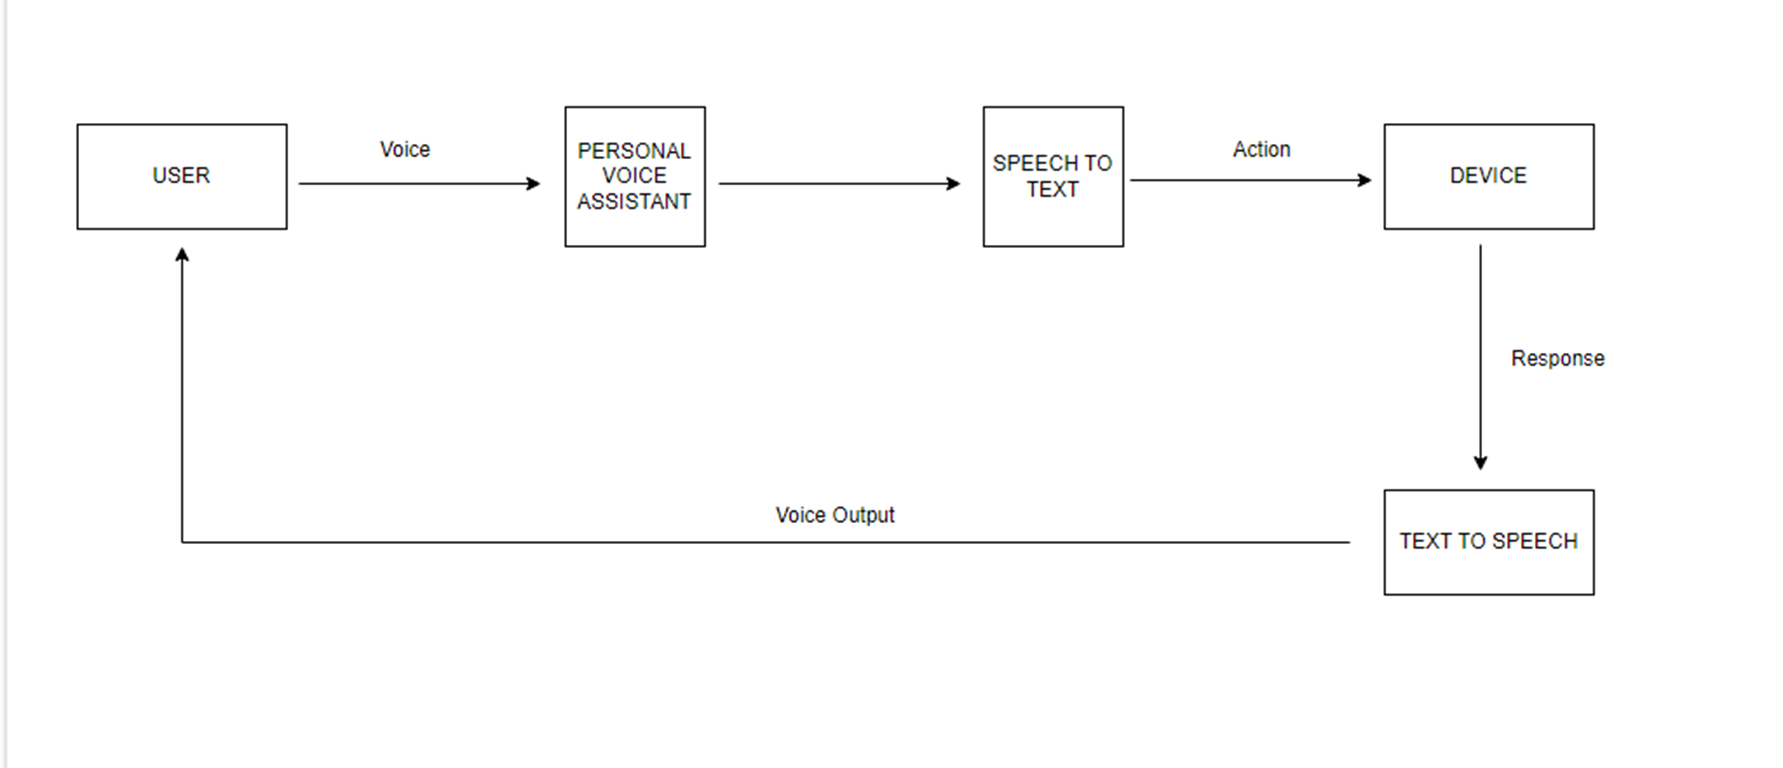
\includegraphics[width=3.5in]{1.png}
\caption{Voice Assistant Architecture Diagram}
\label{fig:diagram}
\end{figure}
Our proposed architecture for file system management using a voice assistant in the Linux ecosystem consists of three main components:
\begin{itemize}
    \item User Interface: The user interface component is responsible for capturing the user's voice commands and converting them into text format. We will use speech-to-text recognition technology to capture and interpret the user's voice commands.

    \item Natural Language Processing (NLP): The NLP component will process the user's text-based commands to identify the user's intent and extract relevant information from the user's command. We will use NLP algorithms to analyze the user's text-based commands.

    \item File System Access: The file system access component will be responsible for accessing and manipulating the files stored in the Linux file system based on the user's commands. We will use Linux system calls to access the file system.
\end{itemize}

Our proposed work will enable users to access and manage files in the Linux file system using a voice assistant, while ensuring user privacy and security. The voice assistant will respond to user commands in a natural and conversational way, allowing users to easily manage their files hands-free.
\vspace{1\baselineskip}

\usetikzlibrary{shapes.geometric, arrows}
\tikzstyle{process} = [rectangle, minimum width=3cm, minimum height=1cm, text centered, draw=black, fill=white]
\tikzstyle{io} = [trapezium, trapezium left angle=70, trapezium right angle=110, minimum width=3cm, minimum height=1cm, text centered, draw=black, fill=white]
\tikzstyle{arrow} = [thick,->,>=stealth]

\begin{figure}
\centering
\begin{tikzpicture}[node distance=2cm]

\node (input) [io] {Voice Input};
\node (nlp) [process, below of=input] {NLP Processing};
\node (output) [io, below of=nlp] {Voice Output};

\draw [arrow] (input) -- (nlp);
\draw [arrow] (nlp) -- (output);

\end{tikzpicture}
\caption{Voice Assistant NLP and Voice Output}
\end{figure}


\section{Voice Assistant Algorithm}
The proposed algorithm for the Voice Assistant involves three main steps: speech recognition, command interpretation, and system interaction. The speech recognition step converts the user's spoken words into text using an Automatic Speech Recognition (ASR) system. The command interpretation step analyzes the text to determine the user's intent and identifies the specific command requested. Finally, the system interaction step performs the requested action on the Linux system by accessing the appropriate system files or executing the appropriate commands. These three steps work together seamlessly to provide a personalized and efficient experience for the user. Given below is the Voice Assistant Algorithm:
\begin{itemize}

\item Import the required modules: pyttsx3, speech-recognition, and os.
\item Initialize the pyttsx3 engine.
\item Set the voice to be used by the pyttsx3 engine.
\item Set the speech rate to a slower pace.
\item Create a recognizer object.
\item Define a function named "gettext()" that uses the microphone as a source for input, listens for the user's input, and tries to recognize the speech using Google Speech Recognition.
\item  Define a function named "filehandling(text)" that takes in the recognized text as an argument and performs file handling operations based on the user's input. The following operations are supported:
\begin{enumerate}
\item Create a file with the given name.
\item List all the files in the current directory.
\item Delete a file with the given name.
\item Call the "gettext()" function to get the user's input.
\end{enumerate}
\item  Speak the recognized text using the pyttsx3 engine.
\item  Call the "filehandling(text)" function to perform the required file handling operation based on the user's input.
\item  Speak the final message "Bye" using the pyttsx3 engine
\end{itemize}

The algorithm consists of several steps for creating a voice assistant for file management. The first step is to import the necessary modules, including pyttsx3, speech-recognition, and os. These modules provide the functionality needed to recognize speech, handle files, and speak the output.

\par Once the modules are imported, the pyttsx3 engine is initialized and the voice and speech rate are set. This ensures that the voice assistant speaks in a clear and understandable manner.

\par Next, a recognizer object is created and a function named "gettext()" is defined. This function listens for the user's input using the microphone and tries to recognize the speech using Google Speech Recognition. The recognized text is then returned.

\par Another function named "filehandling(text)" is defined, which takes in the recognized text as an argument and performs file handling operations based on the user's input. These operations include creating a file with the given name, listing all files in the current directory, deleting a file with the given name, and getting the user's input.

\par The recognized text is then spoken using the pyttsx3 engine, and the "filehandling(text)" function is called to perform the required file handling operation based on the user's input. Finally, the voice assistant speaks the final message "Bye" using the pyttsx3 engine, indicating that the program has ended.

\par Overall, this algorithm provides a high-level overview of the process involved in creating a voice assistant for file management.

\section{Tools Used}
The implementation of the Voice Assistant for file system management in Linux uses several tools and technologies to achieve its functionality. One of the primary tools used is the Python programming language. Python is a widely used high-level programming language known for its simplicity and ease of use.

\par In addition to Python, the implementation also utilizes several Python modules, including Os, Speech Recognition, and Pyttsx. The Os module is a built-in module in Python that provides a way to interact with the operating system, making it ideal for executing file-related commands. The Speech Recognition module is used to recognize and interpret speech input from the user, while Pyttsx is used to enable the feature of voice response in the Voice Assistant.

\par The hardware requirements for the Voice Assistant application are critical to ensure smooth performance of the application. For Windows 10, it is recommended to have an Intel Core i5 or higher processor, as this will ensure that the application runs efficiently. The processor speed and number of cores are important factors to consider when selecting a computer for the Voice Assistant application. A minimum of 4 GB of RAM is also recommended to prevent the system from slowing down when running the application. In addition, it is recommended to have a few GB of free storage space for the proper functioning of the application.

\par For Ubuntu 21.04 or higher, the system requirements are similar to those of Windows 10. The recommended hardware requirements are an Intel Core i5 or higher processor, 4 GB of RAM, and a few GB of free storage space. It is important to note that the system requirements may vary depending on the specific hardware configuration and edition of Ubuntu being used.

\par Apart from the hardware requirements, it is also essential to have a noise-cancelling microphone and a speaker with clear audio output. These peripherals play a crucial role in ensuring the Voice Assistant application can effectively recognize and interpret the user's speech. A noise-cancelling microphone reduces background noise and improves the accuracy of speech recognition, while a clear audio output ensures that the user can hear the responses from the Voice Assistant clearly.

\par Overall, the combination of these tools and technologies makes it possible to create a functional and efficient Voice Assistant for file system management in Linux, providing users with an easy and convenient way to perform file-related tasks using voice commands.


\section{Implementation}
The implementation of the proposed Voice Assistant for file system management in Linux involves using Python programming language and several modules like Os, Speech Recognition, Pyaudio, Pyspeech, and Pyttsx. The system requirements include an operating system like Windows 10 or Ubuntu 21.04 or higher, a modern processor like i5 or higher, at least 4GB of RAM, and a microphone and speaker with clear audio output. The implementation involves developing an algorithm that takes user voice input and executes file management commands like opening, searching, deleting, or listing files. The output is provided in the form of voice responses using the Pyttsx module. The final product aims to provide a private and personalized voice assistant experience with an exclusive focus on user discretion while addressing the security concerns associated with cloud-based voice assistants.
\begin{figure}[h]
\centering
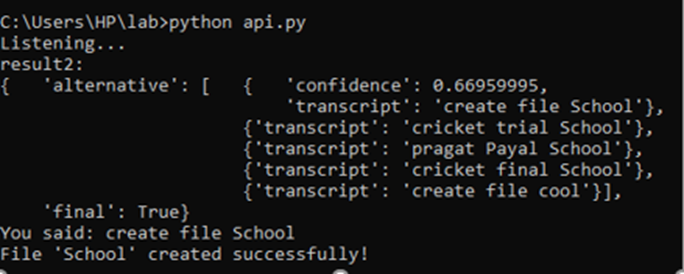
\includegraphics[width=3.5in]{2.png}
\caption{Create File}
\label{fig:diagram}
\end{figure}

\begin{figure}[h]
\centering
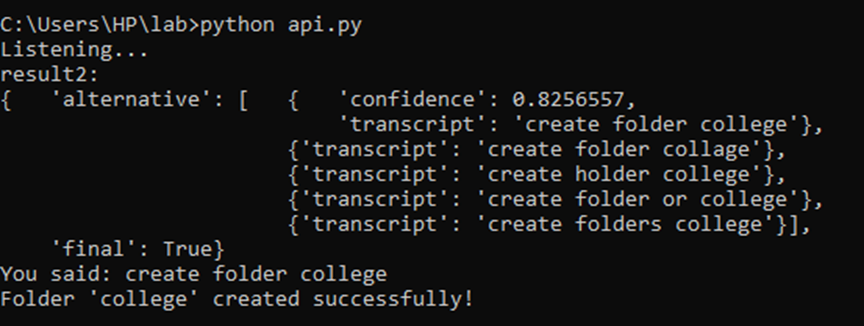
\includegraphics[width=3.5in]{3.png}
\caption{Create Folder}
\label{fig:diagram}
\end{figure}

\begin{figure}[h]
\centering
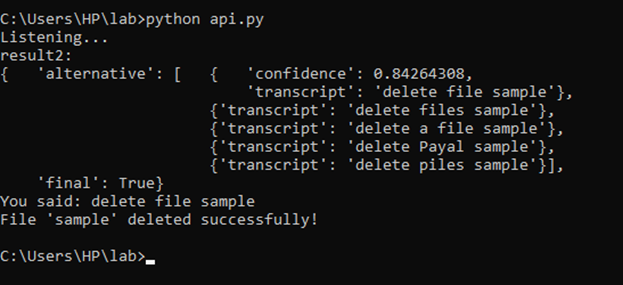
\includegraphics[width=3.5in]{4.png}
\caption{Delete File}
\label{fig:diagram}
\end{figure}

\begin{figure}[h]
\centering
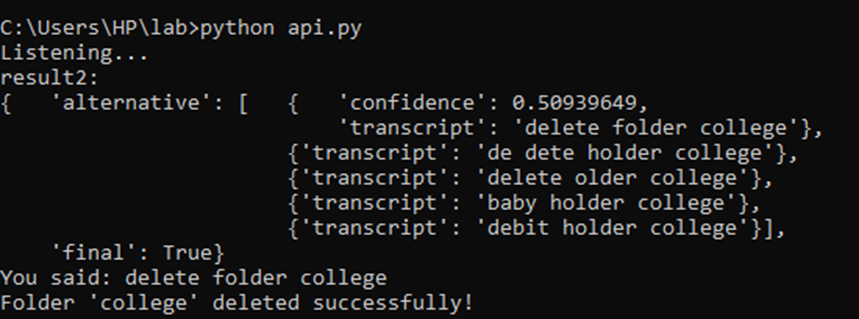
\includegraphics[width=3.5in]{5.png}
\caption{Delete Folder}
\label{fig:diagram}
\end{figure}

\begin{figure}[h]
\centering
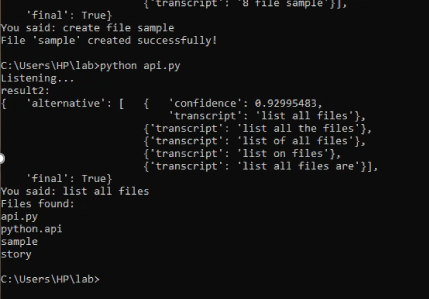
\includegraphics[width=3.5in]{6.png}
\caption{List Files}
\label{fig:diagram}
\end{figure}

The successful implementation of file operations through voice commands using a voice assistant represents a significant step forward in the development of natural language processing technologies. This project showcases the potential of using voice assistants for file system management in Linux, demonstrating the convenience and accessibility of using voice commands to perform file operations. With this implementation, users can perform file operations with ease, saving time and effort, and improving their overall experience.

\section{Conclusion}
In conclusion, the development and successful implementation of a voice assistant for file system management in Linux is a promising step towards making computing more accessible and efficient. The proposed system has the potential to improve the user experience by providing a more intuitive and natural way of interacting with files. The use of advanced technologies like AI and natural language processing has improved the accuracy and effectiveness of the voice assistant.

\par Despite its benefits, there are still concerns related to privacy and security associated with voice assistants. The proposed system runs locally, avoiding the need for streaming audio to cloud service providers, which helps mitigate these concerns. However, there is still a need to ensure that sensitive information is not disclosed or compromised through the use of voice commands. Future research could focus on developing more secure and privacy-focused voice assistant systems.

\par Furthermore, the successful implementation of the proposed voice assistant system for file management in Linux provides a starting point for further research and development in this area. There is a need to explore the potential of voice assistants in other areas, such as healthcare, education, and business. Voice assistants have the potential to revolutionize the way we interact with various devices and services and can help make computing more accessible and inclusive.

\par In summary, the proposed voice assistant system for file management in Linux provides a convenient and efficient way to access files through voice commands. It has potential applications in various fields and can be further developed to improve its effectiveness and security. The successful implementation of this project can serve as a foundation for future research and development in voice assistant technology.

\begin{thebibliography}{20}

\bibitem{christensen2020digital}
Christensen, Anders T and Olesen, Henning and S{\o}rensen, Lene. \emph{"Digital Voice Assistants: A new kind of user agent,"} 2020 13th CMI Conference on Cybersecurity and Privacy (CMI)-Digital Transformation-Potentials and Challenges (51275).

\bibitem{sangpal2019jarvis}
Sangpal, Ravivanshikumar and Gawand, Tanvee and Vaykar, Sahil and Madhavi, Neha.  \emph{"JARVIS: An interpretation of AIML with integration of gTTS and Python,"} 2019 2nd International Conference on Intelligent Computing, Instrumentation and Control Technologies (ICICICT).

\bibitem{subhash2020artificial}
Subhash, S and Srivatsa, Prajwal N and Siddesh, S and Ullas, A and Santhosh, B. \emph{"Artificial intelligence-based voice assistant,"} 2020 Fourth world conference on smart trends in systems, security and sustainability (WorldS4).

\bibitem{akash2022desktop}
Akash, S and Jayaram, Neeraj and Jesudoss, A. \emph{"Desktop based Smart Voice Assistant using Python Language Integrated with Arduino,"} 2022 6th International Conference on Intelligent Computing and Control Systems (ICICCS).

\bibitem{kumar2022voice}
Kumar, Aabhas and Kaur, Damandep and Pathak, Abhishek Kumar. \emph{"Voice Assistant Using Python,"} 2022 International Conference on Cyber Resilience (ICCR).

\bibitem{dinesh2022artificial}
Dinesh, RS Sai and Surendran, R and Kathirvelan, D and Logesh, V. \emph{"Artificial Intelligence based Vision and Voice Assistant,"} 2022 International Conference on Electronics and Renewable Systems (ICEARS).

\bibitem{sati2022intelligent}
Sati, Bhawana and Kumar, Sameer and Rana, Karan and Saikia, Kuhil and Sahana, Subrata and Das, Sanjoy. \emph{"An Intelligent Virtual System using Machine Learning,"} 2022 IEEE IAS Global Conference on Emerging Technologies (GlobConET).

\bibitem{overstreet2019penetration}
Overstreet, Dain and Wimmer, Hayden and Haddad, Rami J. \emph{"Penetration testing of the amazon echo digital voice assistant using a denial-of-service attack,"} 2019 SoutheastCon.

\bibitem{kumaran2020intelligent}
Kumaran, N and Rangaraj, V and Dhanalakshmi, R and others. \emph{Intelligent Personal Assistant-Implementing Voice Commands enabling Speech Recognition,"} 2020 International conference on system, computation, automation and networking (ICSCAN).

\bibitem{iannizzotto2018vision}
Iannizzotto, Giancarlo and Bello, Lucia Lo and Nucita, Andrea and Grasso, Giorgio Mario. \emph{"A vision and speech enabled, customizable, virtual assistant for smart environments,"} 2018 11th International Conference on Human System Interaction (HSI).

\bibitem{de2022voice}
De, Shilpa and Kumar, Vishwas and Reddy, Ram. \emph{"Voice-Assistant Liveness Analysis,"} 2022 IEEE Silchar Subsection Conference (SILCON).

\bibitem{rajakumar2022iot}
Rajakumar, P and Suresh, K and Boobalan, M and Gokul, M and Kumar, G Darun and Archana, R. \emph{"IoT Based Voice Assistant using Raspberry Pi and Natural Language Processing,"} 2022 International Conference on Power, Energy, Control and Transmission Systems (ICPECTS).

\bibitem{buchta2022nux}
Buchta, Karolina and W{\'o}jcik, Piotr and Nakonieczny, Konrad and Janicka, Justyna and Igras-Cybulska, Magdalena. \emph{"NUX Characters-interaction with voice assistants in Virtual Reality,"} 2022 IEEE International Symposium on Mixed and Augmented Reality Adjunct (ISMAR-Adjunct).

\bibitem{yadlapally2023review}
Yadlapally, Dhanush Kumar and Vasireddy, Bhavana and Marimganti, Madhumitha and Chowdary, Teja and Karthikeyan, C and Vignesh, T. \emph{"A Review on the Potential of AI Voice Assistants for Personalized and Adaptive Learning in Education,"} 2023 7th International Conference on Computing Methodologies and Communication (ICCMC).

\bibitem{klein2020measuring}
Klein, Andreas M and Hinderks, Andreas and Schrepp, Martin and Thomaschewski, J{\"o}rg. \emph{"Measuring user experience quality of voice assistants,"} 2020 15th Iberian Conference on Information Systems and Technologies (CISTI).

\bibitem{rajkumarpillay2022implementing}
RajkumarPillay, D and Binda, MB and Krishna, ManamVamsi and Saravanan, A and Raja, Archana and Saxena, Pankaj. \emph{"Implementing an Artificial Intelligence based Ideal form of Virtual Personal Assistant Design for Various Communication Medium,"} 2022 3rd International Conference on Electronics and Sustainable Communication Systems (ICESC).

\bibitem{swamy2022voice}
Swamy, Tata Jagannadha and Nandini, M and Nandini, B and Anvitha, V Laxmi and Sunitha, Ch and others. \emph{"Voice and Gesture based Virtual Desktop Assistant for Physically Challenged People,"} 2022 6th International Conference on Trends in Electronics and Informatics (ICOEI).

\bibitem{shang2020voice}
Shang, Jiacheng and Wu, Jie. \emph{"Voice liveness detection for voice assistants using ear canal pressure,"} 2020 IEEE 17th International Conference on Mobile Ad Hoc and Sensor Systems (MASS).

\bibitem{vassilev2020two}
Vassilev, Vassil and Phipps, Anthony and Lane, Matthew and Mohamed, Khalid and Naciscionis, Artur. \emph{"Two-factor authentication for voice assistance in digital banking using public cloud services,"} 2020 10th International Conference on Cloud Computing, Data Science \& Engineering (Confluence).

\bibitem{ahmed2022mfcc}
Ahmed, Syed Fahad and Jaffari, Rabeea and Ahmed, Syed Saad and Jawaid, Moazzam and Talpur, Shahnawaz. \emph{"An MFCC-based Secure Framework for Voice Assistant Systems,"} 2022 International Conference on Cyber Warfare and Security (ICCWS).

\end{thebibliography}

\bibliographystyle{IEEEtran}

\end{document}
